\begin{figure}[t]
\centering
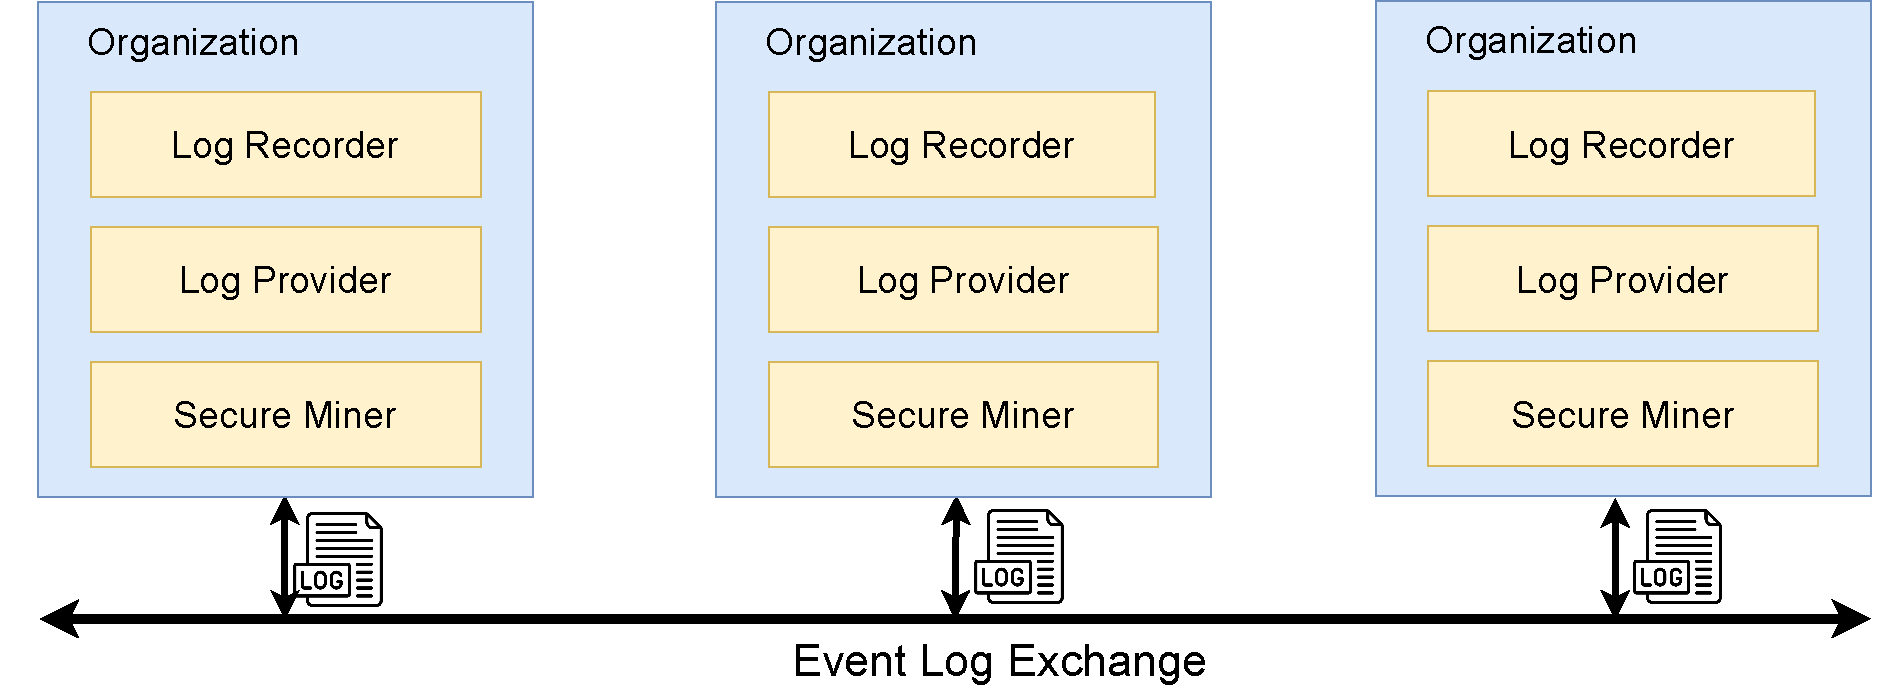
\includegraphics[width=11cm]{content/figures/architecture_diagram.pdf}
\caption{High-level architectural overview.}
\label{fig:architecture_diagram}
\end{figure}
In this section, we present the high-level architecture underlying our solution. We take into account the main functionalities of each component avoiding details on the employed technologies discussed in the next sections. Once introduced the architecture, we focus on the \texttt{Secure Miner} component that represent the core of our contribution.

\subsection{Architecture at large}
Our architecture involves networks of nodes controlled by different \texttt{Organization}s exchanging their event logs. \texttt{Organization}s in the same network collaborate to achieve a common objective and compose business processes whose event logs are scattered across multiple places. Therefore, each \texttt{Organization} produces event logs recording the operations executed to complete a business process. The hospital, the specialized clinic, and the pharmaceutical company mentioned in the running example provide an example of partner \texttt{Organization}s. An \texttt{Organization} may assume one of the following two different roles or both: \textit{provider}, if it delivers local event logs to be collaboratively mined; a \textit{miner} whenever it applies process mining algorithms using local event logs in combination with ones generated by providers. %Each \texttt{Organization} is associated with an asymmetric public/private key pair through which it authenticates messages sent to other \texttt{Organizations}.

In \cref{fig:architecture_diagram}, we propose a high level schematization of our solution. Each \texttt{Organization} embeds four main components, which we describe next: the \texttt{Log Recorder}, the \texttt{Log Provider} and the \texttt{Secure Miner}.

The maintenance of event logs is the core task performed by \texttt{Log Recorder}. This component registers the events taking place in the \texttt{Organization}. The \texttt{Log Recorder} is queried by the local \texttt{Log Provider} for event logs to be fed into \texttt{Secure Miner}s. 

% \subsubsection{PAIS Interface.}
%The \texttt{PAIS Interface} collects the logic to interact with the Process-aware Information Sytem (\texttt{PAIS}) of the \texttt{Organization}. \texttt{PAIS} systems help \texttt{Organization}s to handle business processes including accounting and resource management. The maintenance of event logs is the core tasks performed by these systems~\cite{Dumas.etal/2018:FundamentalsofBPM}. In our architecture, we generalize the interaction with \texttt{PAIS}s through the \texttt{PAIS Interface}. The \texttt{PAIS Interface} is queried by the local \texttt{Log Provider} for event logs to be fed into \texttt{Secure Miner}s. 


% \subsubsection{Log Provider.}
The \texttt{Log Provider} component delivers on-demand data to \texttt{Secure Miner}s. % belonging to partner \texttt{Organization}s. 
It controls access to owned event logs by authenticating data requests generated by miners. \texttt{Log Provider}s reject demands from unauthorizated parties and only permit \texttt{Secure Miners} of partner \texttt{Organizations} to use the data.    %\texttt{Log Provider}s authenticate event log requests 
 %The goal of the authentication procedure is to extract the public key representing the identity of the sending \texttt{Secure Miner}.

The \texttt{Secure Miner} shelters external event logs inside an \texttt{Organization}'s system by preserving data confidentiality and integrity. We provide an in deepth focus on this component as follow.

\begin{figure}[t]
\centering
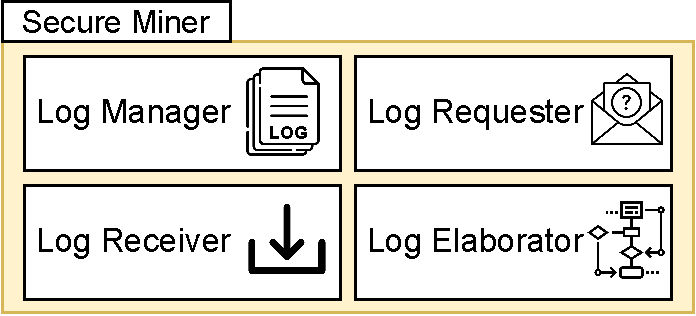
\includegraphics[width=7 cm]{content/figures/secure_miner.pdf}
\caption{Modules of the Secure Miner component.}
\label{fig:trusted_miner}
\end{figure}




\subsection{Secure Miners}
%The \texttt{Secure Miner} is a trusted application running inside the \texttt{Reserved Zone} that makes its source code and data tamper-proof. 
The primary objective of the \texttt{Secure Miner} is to allow \texttt{Organization}s to execute process mining algorithms using %local event logs alongside 
event logs retrieved from partner \texttt{Organization}s, ensuring fair data utilization to log providers. \texttt{Secure Miner}s leverage isolated execution contexts that guarantee tamperproofing and data confidentiality. In \cref{fig:trusted_miner}, we show an high level schematization of \texttt{Secure Miner}s in which we distinguish four different modules: the \texttt{Log Manager}, the \texttt{Log Requester}, the \texttt{Log Receiver}, and the \texttt{Log Elaborator}

Event logs belonging to partner \texttt{Organizaition}s are stored in the isolated execution context of the \texttt{Secure Miner}. We handle these data via the \texttt{Log Manager} that makes event log access not practicable from outside the \texttt{Secure Miner}'s execution context. Thus, the \texttt{Log Manager} prevents external parties from having direct access to event logs. These unauthorized entities include the owner of the miner \texttt{Organization} system. %Therefore, the \texttt{Log Manager} hinders direct access to event logs to parties external to the \texttt{Secure Miner}, including the owner of the miner \texttt{Organization} system. %Modules of the \texttt{Secure Miner} are the only entities enabled to access data controlled by the \texttt{Log Manager}. %Referring to our motivating scenario, the only way for the hospital to use the event logs retrieved from the specialized clinic is via the secure procedures offered by its \texttt{Secure Miner}.

The \texttt{Log Requester} and the \texttt{Log Receiver} are the fundamental modules that we employee during the event log exchange. \texttt{Log Requester}s initalize the exchange procedure and sends authenticable data requests to the \texttt{Data Provision} module of log providers. The \texttt{Log Receiver} collects event logs sent by \texttt{Log Providers} and entrust them to the \texttt{Log Manager}. When collecting data, \texttt{Log Receiver}s prove their trustworthiness to \texttt{Log Provider}s delivering evidences that certifies the \texttt{Secure Miner}'s execution context.% According to our running example, the hospital's \texttt{Log Receiver} must prove its trusted nature to the clinc and the pharmaceutical company's \texttt{Log Provider} before receiving event logs, showing that it is actually running in a \texttt{Reserved Zone}.

The \texttt{Log Elaborator} is the core module of the \texttt{Secure Miner}. It collects the logic to safely execute process mining algorithms. It support the integration of \textit{process discovery}~\cite{citation}, \textit{conformance checking}~\cite{citation} and \textit{performance analysis}~\cite{ciation} tecniques. When activated, the \texttt{Log Elaborator} %interacts with the \texttt{Log Manager} in order to 
accesses external event logs inside the \texttt{Secure Miner} and integrates them with the local event log of the \texttt{Organization}. We refer to this procedure as \textit{merging}. %These are integrated with the local event log by the \texttt{Log Elaborator} via the merging procedure.
During the merging, the \texttt{Log Elaborator} enriches local traces with events belonging to logs from partner \texttt{Organization}s.







\begin{comment}
\subsection{Workflow}
% \label{sec:architecture:workflow}
\subsubsection{Initialization}
\subsubsection{Data Exchange}
%The goal of the authentication procedure is to extract the public key representing the identity of the sending \texttt{Secure Miner}.
%Remote Attestation and Log Segmentation are crucial procedures handled by the \texttt{Log Provider} during the provision process. Through Remote Attestation, \texttt{Log Provider}s verify that the \texttt{Secure Miner} that has generated the log request  is: (i) a known software object running inside a Reserved Zone; (ii) controlled by a partner \texttt{Organization} that has rights to access the event log. We named Log Segementation the process through which \texttt{Log Provider}s split the event log to be delivered in sub-log of smaller size.
\subsubsection{Data Elaboration}


\end{comment}
